\item \textbf{{[}ACJC/PRELIM/9569/2021/P2/Q2{]} }

An $\mathtt{n\times n}$ chessboard consists of an $\mathtt{n\times n}$
grid of small squares. For this task, the squares are numbered using
a coordinate system as a tuple of two integers. The first integer
is the column number, starting from \texttt{1} at the left, and the
second integer is the row number, starting from \texttt{1} at the
bottom.

A chess knight is a piece that occupies a square, and can then move
to another square according to one of the following rules:
\begin{itemize}
\item moving two squares horizontally and then one square vertically in
either direction, or 
\item moving two squares vertically and then one square horizontally in
either direction.
\end{itemize}
See the diagram below for examples.
\begin{center}
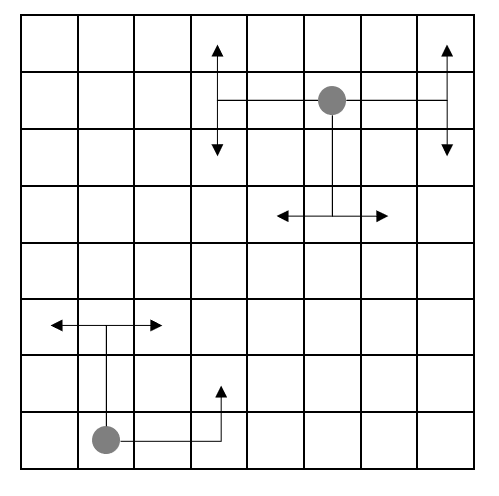
\includegraphics[width=0.5\paperwidth]{C:/Users/Admin/Desktop/Github/question_bank/LyX/static/img/9569-ACJC-2020-P2-Q2}
\par\end{center}

The knight at \texttt{(2,1)} can move to \texttt{(1,3)}, \texttt{(3,3)}
or \texttt{(4,2)}. 

The knight at \texttt{(6,7)} can move to \texttt{(4,6)}, \texttt{(4,8)},
\texttt{(5,5)}, \texttt{(7,5)}, \texttt{(8,6)} or \texttt{(8,8)}.

Only the starting and ending squares of the knight\textquoteright s
move are counted as being visited by the knight, and not the squares
that the knight passes over while moving.

A knight\textquoteright s tour is a sequence of moves that a chess
knight makes on a chessboard, so that it visits every square of the
chessboard exactly once. It does not need to return to its starting
square.

\subsubsection*{Task 2.1}

For a given value of \texttt{n} and a list of squares, write program
code to determine if the list is a knight\textquoteright s tour of
an $\mathtt{n\times n}$ chessboard.

Test your code using the values\texttt{ $\mathtt{n=7}$} and the list
of squares given in the files: 
\begin{itemize}
\item \texttt{TASK2TOUR.txt}, which is a valid tour; 
\item \texttt{TASK2NOTOUR.txt}, which is not a valid tour. \hfill{}{[}10{]}
\end{itemize}
An algorithm to generate a knight\textquoteright s tour needs to keep
track of the squares already visited, so that the knight does not
visit them a second time during the tour.

\subsubsection*{Task 2.2}

Suppose the knight is currently on square square, and a list of squares
already visited by the knight is given in \texttt{lis}.

Write a function \texttt{available(square,lis)} that returns a list
of squares which the knight can visit on its next move from \texttt{square},
and are not currently in \texttt{lis}. These are the squares available
to the knight as it tries to complete the tour.

The output should be given in lexicographic order, that is, with the
column numbers in ascending order, and, among the squares with the
same column number, with the row numbers in ascending order. \hfill{}{[}6{]}

\subsubsection*{Task 2.3}

The knight starts at \texttt{(1,1)}, the bottom left square, of an
$8\mathtt{\times}8$ chessboard.

From each square, the knight moves to the available square from which
it has the smallest number of available squares after that. If there
is a tie, the square which comes first in lexicographic order is chosen.

Write program code to generate the knight\textquoteright s tour as
a list of squares in the order they are visited.

Download your program code and output for Task 2 as \texttt{TASK2\_<your
name>\_<centre number>\_<index number>.ipynb}\hfill{} {[}9{]}